\documentclass{chi-ext}
% Please be sure that you have the dependencies (i.e., additional LaTeX packages) to compile this example.
% See http://personales.upv.es/luileito/chiext/

\copyrightinfo{
  Copyright is held by the author/owner(s).\\
  \emph{MOBILEHCI'14}, April 27 -- May 2, 2013, Toronto, Canada.\\
  ACM 978-1-XXXX-XXXX-X/XX/XX.\\
}

\title{Simple Visual and Vibrotactile Patterning within Transmedia Gaming Experiences}

\numberofauthors{5}
% Notice how author names are alternately typesetted to appear ordered in 2-column format;
% i.e., the first 4 authors on the first column and the other 4 authors on the second column.
% Actually, it's up to you to strictly adhere to this author notation.
\author{
  \alignauthor{
  	\textbf{Adam Tindale}\\
  	\affaddr{OCAD University}\\
  	\affaddr{Toronto, ON M5T 1W1 Canada}\\
  	\email{atindale@faculty.ocadu.ca}
  }\alignauthor{
  	\textbf{Jessica Peter}\\
  	\affaddr{OCAD University}\\
  	\affaddr{Toronto, ON M5T 1W1 Canada}\\
  	\email{jp11jg@student.ocadu.ca}
  } 
    \vfil
  \alignauthor{
  	\textbf{Michael Cumming}\\
  	\affaddr{OCAD University}\\
  	\affaddr{Toronto, ON M5T 1W1 Canada}\\
  	\email{mcumming@ocadu.ca}
  }\alignauthor{
  	\textbf{Sara Diamond}\\
  	\affaddr{OCAD University}\\
  	\affaddr{Toronto, ON M5T 1W1 Canada}\\
  	\email{sdiamond@ocadu.ca}
  }
    \vfil
    \alignauthor{
  	\textbf{Hudson Pridham}\\
  	\affaddr{OCAD University}\\
  	\affaddr{Toronto, ON M5T 1W1 Canada}\\
  	\email{hp12pk@student.ocadu.ca}
  } 
}


% Paper metadata (use plain text, for PDF inclusion and later re-using, if desired)
\def\plaintitle{Simple Visual and Vibrotactile Patterning within Transmedia Gaming Experiences}
\def\plainauthor{Adam Tindale}
\def\plainkeywords{pattern recognition, wearable devices, gaming, transmedia, multi-sensory, vibrotactile}
\def\plaingeneralterms{Gaming, Patterns, Transmedia}

\hypersetup{
  % Your metadata go here
  pdftitle={\plaintitle},
  pdfauthor={\plainauthor},  
  pdfkeywords={\plainkeywords},
  pdfsubject={\plaingeneralterms},
  % Quick access to color overriding:
  citecolor=black,
  linkcolor=blue,
  menucolor=black,
  urlcolor=blue,
}

\usepackage{graphicx}   % for EPS use the graphics package instead
\usepackage{balance}    % useful for balancing the last columns
\usepackage{bibspacing} % save vertical space in references

\begin{document}

\maketitle

\begin{abstract}
In this paper we describe a series of demo experiences focusing on the communication of information through low resolution vibrotactile and LED displays.

Transmedia games are notable for the possibilities they afford for rich multimedia narratives and innovative ways of integrating and switching between diverse media types. Simple, wearable devices are a promising way of encouraging participation with those who consume and contribute towards transmedia narratives. In this paper we explore techniques for adding simple visual and vibro-tactile patterning for children aged 8-12, which add sensory interest to gameplay as well as convey useful information about basic game dynamics and expected user interactions.
\end{abstract}

\keywords{\plainkeywords}
\textcolor{red}{Mandatory section to be included in your final version.}

\category{H.5.m}{Information interfaces and presentation (e.g., HCI)}{Miscellaneous}. 
%See \cite{ACMCCS} 
See: \url{http://www.acm.org/about/class/1998/} 
\textcolor{red}{Mandatory section to be included in your final version.}

\terms{\plaingeneralterms}
\textcolor{red}{Optional section to be included in your final version.}


\section{Introduction}
% ======================================================================
This project involves adding simple user involvement and user participation to complex transmedia narratives. Transmedia narratives are by their nature complex and multisensory \cite{phillips_creators_2012}. If well done they engage viewers and can build interesting emergent social cohorts. They have the potential of explaining and making connections between complex concepts in a fluid and graceful way. Yet, such narratives demand a high level of skill in their artistic conception and organization. 

Users wish to interact with these narratives in order to direct the narrative, to provide information demanded by the game and to acknowledge that have sufficient involvement to proceed in the game. Such interactions could easily be confusing and counter-productive to the flow of the narrative. 

Adding complex user interaction on top of the sometimes challenging demands of transmedia is likely be unsuccessful and confusing to its audience. 

Our demo experiences focus on an attempt to make the interactions very simple, such that they convey information in a way that presents few cognitive demands on the user and which the user would tend to find enjoyable and engaging?even if they were not participating in a transmedia game. 

% ======================================================================
\section{Background}
% ======================================================================

\subsection{Haptics in general}
Ruspini provides a useful introduction to the concepts and history of haptics, the basics of haptic psychophysics and haptic devices past and present \cite{ruspini1999haptics}.

MacLean \cite{maclean2009putting} discusses the potential benefits of haptic feedback as an ambient notification system. Unlike visual information, which can be obtrusive while completing a task, or sound, which can be obnoxious in a public environment, haptic feedback is usually experienced only by the user and does not directly interfere with the task at hand. 

Oliveira and Maciel propose a network of haptic actuators that use a set of patterns to express elements of an environment that has obstacles and free paths and demonstrates the use of a haptic language that helps users navigate and consists of vibrotactile signs to complement or replace their vision. \cite{deusing}

In Profita (2013) \cite{profita2013don} researchers reveal the results of studies completed in the United States and South Korea on the social acceptability of interacting with on-body controllers in which participants  ranked factors such as ?awkwardness? and ?coolness? of the exhibited interactions as actors performed them. This article is helpful for providing insight on social acceptability of wearable positioning as it relates to gender and culture.

De Jesus Oliveira and Maciel \cite{deusing} present research towards building a hand-mounted array of haptic actuators intended to help the wearer perform a variety of tasks including orientation. They propose that the actuators could be connected to environment-aware sensors so that the actuators would vibrate in a set pattern to alert the wearer of an obstacle (or help instruct them to perform a certain task). Such haptic systems could help visually impaired users navigate. They would also enable fully sighted users to perform certain tasks without being distracted by personal technologies (i.e. using a smartphone to check a map).

\subsection{Low resolution haptic arrays for use in conveying information}
Low resolution arrays can be useful in indicating directionality and intensity of stimuli. They can also be easily programmed to indicate various game modes. 


% ======================================================================
\section{Prototypes}
% ======================================================================

\subsection{Introduction to prototypes}
Prototypes began as the simplest and least refined expression of a wearable or functional haptic device. The first prototype has simple linear arrangement of LED light and mobile phone type vibrating motors. When the connected to an Arduino micro-controller this band emits a rhythmic and visual sequential pattern that could conceivably could be used to notify band wearers of others in their vicinity. Although this band was perhaps the most simplistic band possible, it could in fact be functional in some minimal sense for a transmedia gaming experience. Also, such a minimal band would be inexpensive to manufacture and simple to program. 

\subsection{Use cases for prototypes}
We have identified three important use cases: 1. Detect other band wearers (wirelessly) who happen to be in the vicinity, 2. Give something of value to another wearer, 3. Exchange something of value with another wearer and 4. Give the wearer some indication of the game mode the wearer is in.

\begin{figure}
  \begin{center}
  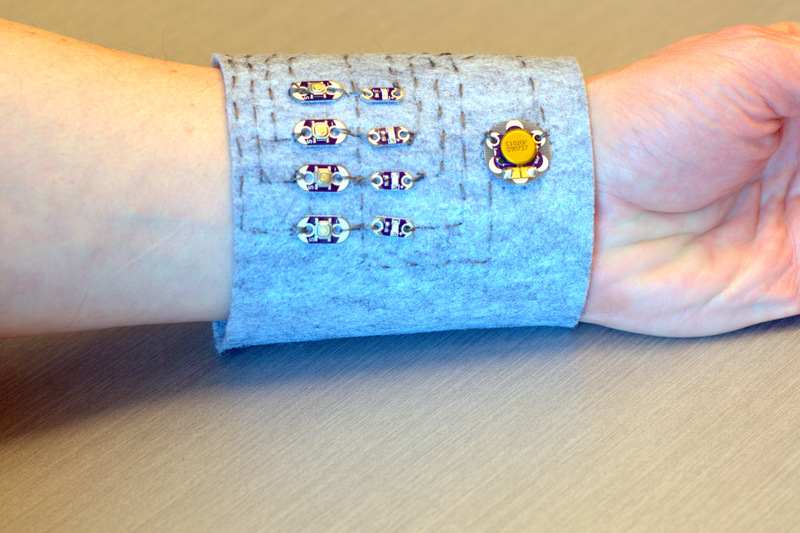
\includegraphics[width=\columnwidth]{images/P1130375.jpg}
  \caption{A wearable interface.}
  \label{fig:marginparsample}
  \end{center}  
\end{figure}

\begin{figure}
  \begin{center}
  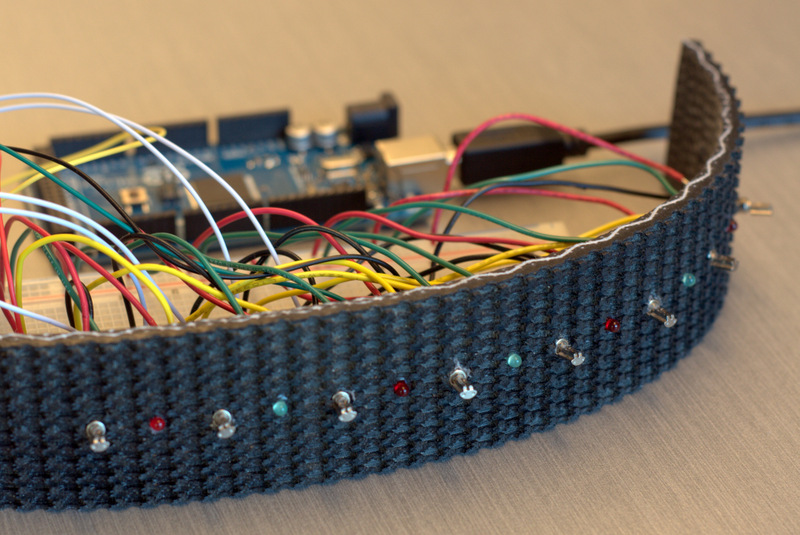
\includegraphics[width=\columnwidth]{images/P1130386.jpg}
  \caption{A simple wearable device prototype that features visual and vibrotactile sensory outputs.}
  \label{fig:rubberVibeBand01}
  \end{center}  
\end{figure}

\section{Conclusions}
Transmedia narrative are technical constructions, but they are also depend on subtle artistic  techniques that switch between narratives in a seamless and fluid manner. We believe that the final quality of a transmedia narrative ultimately depends on this kind of artistic judgement.

\section{Future Work}
Wearable devices and associated technologies for developing is developing at a rapid pace.
Miniaturization, bearability and functionality is obviously a primary concern of such devices. 

\section{Acknowledgements}
%We thank the valuable input from Patrick Crowe and all those at Xenophile Media Inc. who have great expertise in crafting transmedia narratives; Dr. Rachel Zuannon from the Graduate Design Program at Anhembi Morumbi University, Sao Paulo, Brazil.; the professors, students and staff within OCAD University's Digital Futures Initiative (DFI) for their valuable input and helpful comments. The following students within the DFI program worked on this project over many months: Hudson Pridham, Ryan Maksymic, Jessica Peter and Boris Kourtoukov. We thank Dr. Steve Szigeti for his contributions to this project and we especially thank Dr. Sara Diamond, President of OCAD University for her guidance and support.

We would like to thank Ryan Maksymic, Boris Kourtoukov, and Steve Szigeti for their help in the development of this project. This work is generously supported by grants from the Natural Sciences and Engineering Research Council of Canada (NSERC), International Science and Technology Partnerships Canada.

\balance
\bibliographystyle{acm-sigchi}
\bibliography{MGDSPET}

\end{document}
